\documentclass[../summary.tex]{subfiles}

\begin{document}
	
	\section{Philosophy of science}
	
	\subsection{Role of human activity in climate change}
	
	We can ask ourself the question whether or not climate change is due to human activities. The answer to that question has changes over time due to a progressive understanding over the years as a result of climate research worldwide. Figure \ref{fig:progressive-understanding-climate-change} shows the evolution of this understanding. At this moment, it is unequivocal that human influence has warmed the atmosphere, ocean and land, but this clearly was not always the case.
	
	\begin{figure} [htbp]
		\centering
		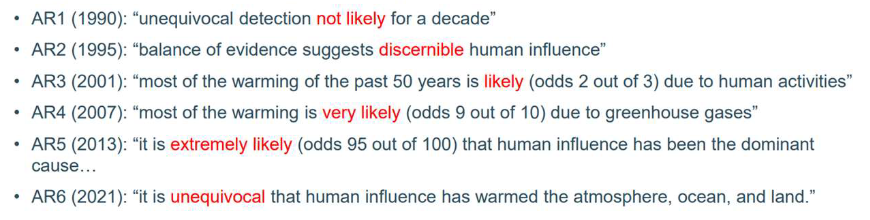
\includegraphics[width=1\linewidth]{images/progressive-understanding-climate-change.png}
		\caption{Evolution of climate change understanding}
		\label{fig:progressive-understanding-climate-change}
	\end{figure}
	
	\subsection{The Precautionary Principle}
	
	The Rio Declaration of 1992 states that where there are threats of serious or irreversible damage, lack of full scientific certainty shall not be used as a reason for postponing cost-effective measures to prevent environmental degradation. This is known as the \textbf{Precautionary Principle} (\textit{het Voorzorgsprincipe}).
	\\\\
	Now what exactly is \textbf{full scientific certainty}? The ideal type of science is based on \textbf{reliable and rational knowledge} and not merely intuitive or emotional. Secondly, science should be \textbf{generalisable}. There can be no exceptions and it should be also valid for future, unknown cases. Space and time are uniform and science can not be merely anecdotic or casuistic. Furthermore, science should be \textbf{objective} and based on facts instead of interests. Science should also be \textbf{coherent} and can't be a loose set of statements. Lastly, there should be a \textbf{consensus in scientific community}. 
	
	\subsection{Demarcation criteria}
	
	Next, we will discuss what the criteria are to distinguish science from non-science. We call this the \textbf{demarcation criteria}. At first sight, the use of numbers and mathematics looks like a logical criterion. However, there are a lot of non-science domains that also use numbers, think of the score of a football game for example. On the other hand, there are also science-domains that don't use really use numbers, like psychology for instance. A second criterion could be the possibility to make prognoses or to do experiments. But how precise must these prognoses then be to be considered science? And what if there are practical or ethical objections to do a certain experiment? We can conclude that these criteria also aren't ideal. A last possible criterion is whether it can be verified or falsified. The origin of verifiability as a demarcation criterion lays in "logical empiricism". We can look at science as a set of true sentences. This can be an empirical or a logical truth. We can decompose the sentences in their constituent parts and check for each part whether it is either a logical operator, or whether is is verifiable.
	
\end{document}